\section{LiDAR generation and requirements}
\label{sec:rq2}

Applying generation methods to automotive LiDAR requires reproducing an
observation of a scene, rather than its geometry alone. The sensor samples
visible surfaces, so beam directions, \gls{occlusion} and missing returns
influence the resulting \gls{point-cloud}. Training data must also associate
these measurements with annotations appropriate to the perception task
\parencite{manivasagamLiDARsimRealisticLiDAR2020,
xiaoTransferLearningSynthetic2022}.
The following comparison examines how virtual environments, reconstructed
assets and learned scan models address these requirements, and where each
approach retains dependence on real data.

\subsection{Virtual scenes and generated annotations}

Virtual environments provide access to scene geometry and object identity,
which can be used to generate measurements together with annotations.
PreSIL illustrates this approach by deriving scans from GTA~V depth data,
avoiding the simplified collision geometry used by the game. However, its
released point clouds have a forward-facing field of view and omit
reflectance and motion distortion
\parencite{hurlPreciseSyntheticImage2019}.
These choices show that access to detailed virtual geometry does not ensure
that all properties of the target sensor are reproduced. Their relevance
depends on the intended use, particularly whether the perception model
requires intensity information or observations outside that field of view.

SynLiDAR extends the virtual-scene approach to semantic segmentation with
32 annotated classes. Its intensity model uses real SemanticKITTI data,
while its point cloud translator (PCT) separately addresses differences in
appearance and sparsity \parencite{xiaoTransferLearningSynthetic2022}.
Thus, generated annotations can reduce manual labelling without removing
real-data requirements from the complete pipeline. Moreover, source labels
must be mapped to the target dataset's classes before training and
comparison. PreSIL and SynLiDAR therefore illustrate complementary
requirements: the observation model must supply suitable sensor features,
and the annotation scheme must match the learning task.

\subsection{Reconstructed scenes and hybrid sensor modelling}

Reconstruction-based simulation obtains scene assets from real recordings
rather than relying entirely on virtual assets. LiDARsim reconstructs maps
and vehicles, composes scenes from these assets, and combines
\gls{ray-casting} with learned \gls{ray-drop}
\parencite{manivasagamLiDARsimRealisticLiDAR2020}.
Figure~\ref{fig:lidarsim-pipeline} illustrates the two stages. The upper
panels show how accumulated observations are completed and refined into a
\gls{surfel} asset. The lower panels compare ray-cast measurements,
measurements after learned ray drop, and a real scan. Together, they
explain why reconstructing an object's surface and modelling which returns
a sensor records are separate parts of the generation process.

\begin{figure}[htbp]
\centering
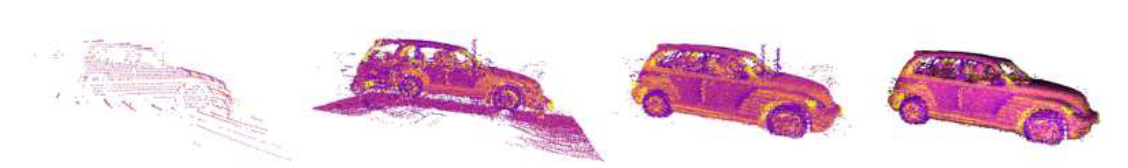
\includegraphics[width=.68\linewidth]{Images/IndividualLidarSweep to surfelmeshing.png}

\vspace{1mm}
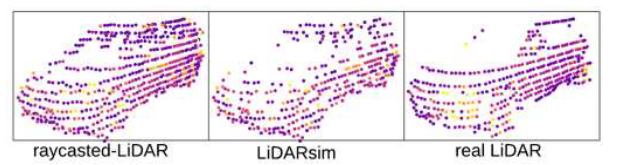
\includegraphics[width=.50\linewidth]{Images/RaycastvsLiDARsimvsRealLiDAR.png}
\caption{Asset reconstruction and sensor modelling in LiDARsim.
Top: an individual sweep, accumulated observations, symmetry completion,
and the refined surfel asset. Bottom: ray-cast measurements, measurements
with learned ray drop, and real LiDAR observations.
Reproduced from Figures~4 and~7 of Manivasagam et al.
\parencite{manivasagamLiDARsimRealisticLiDAR2020}.
The panels illustrate changes in geometry and sampling. Training utility
requires separate evaluation on real data.}
\label{fig:lidarsim-pipeline}
\end{figure}

This approach permits controlled scene composition while retaining
geometric detail from real observations. Its coverage nevertheless depends
on the reconstructed assets, and the demonstrated vehicle reconstruction
does not establish equivalent support for deformable road users
\parencite{manivasagamLiDARsimRealisticLiDAR2020}.
Consequently, realistic individual assets should not be equated with
coverage of all relevant traffic participants or configurations.

\subsection{Learned scans and conditional completion}

Learned scan generation shifts the modelling emphasis from explicit scene
assets to the distribution of sensor observations. LiDARGen represents
range and intensity in \glspl{range-image}, using stochastic denoising to
generate scans and conditional \gls{densification} to complete sparse
inputs. Its KITTI-360 and nuScenes experiments use sensor-specific angular
representations \parencite{zyrianovLearningGenerateRealistic2022}.
This representation captures the organisation of measurements, but does
not itself provide object identities, semantic labels or an editable scene.
Furthermore, completing an existing scan retains information from that
input, whereas unconditional generation samples a new observation.
These capabilities serve different purposes, so evidence for completion
must be distinguished from evidence that generated scans can train a
perception model.

\subsection{Requirements across generation pipelines}

Table~\ref{tab:lidar-generation-comparison} summarises the practical
consequences of these design choices. Scene-based methods provide access
to geometry and annotations, but require suitable observation models.
Learned methods capture scan patterns, while labels and scene control
remain additional requirements. Hybrid methods connect these capabilities
without eliminating dependence on real recordings.

\begin{table}[htbp]
\caption{Comparison of the reviewed LiDAR generation pipelines.
Entries summarise capabilities and constraints, rather than rank
perception performance.}
\label{tab:lidar-generation-comparison}
\small
\begin{tabularx}{\linewidth}{@{}lYY@{}}
\toprule
\textbf{Method} & \textbf{Generation basis} & \textbf{Key requirement or constraint} \\
\midrule
PreSIL \parencite{hurlPreciseSyntheticImage2019}
& Virtual scenes with generated annotations
& Forward-facing scans without reflectance or motion distortion. \\
SynLiDAR \parencite{xiaoTransferLearningSynthetic2022}
& Virtual scenes with semantic labels
& Real data for intensity modelling and class mapping for transfer. \\
LiDARsim \parencite{manivasagamLiDARsimRealisticLiDAR2020}
& Reconstructed assets with learned ray drop
& Real recordings and annotations for asset construction and sensor modelling. \\
LiDARGen \parencite{zyrianovLearningGenerateRealistic2022}
& Learned range and intensity distributions
& Example scans for learning. Semantic labels are not generated by the scan model. \\
\bottomrule
\end{tabularx}
\end{table}

Across these pipelines, scene diversity describes what is observed,
whereas sensor modelling determines how it is sampled. Paired-scenario
experiments identify material response, scanning motion and
traffic-participant geometry as contributors to the \gls{domain-gap}
\parencite{manivasagamZeroDomainGap2023}.
The implication is that scene coverage, sensor behaviour and annotation
consistency must be assessed together. Visual similarity can reveal
sampling differences, as the LiDARsim example illustrates, but cannot
establish whether generated data improves perception on real measurements.
The next section therefore examines how evaluation connects these data
properties to performance on real perception tasks.
